\section{Transfer Learning}
\label{sec:transfer_learning}

Due to the complex nature of visual reasoning, it appears that
transfer learning from a source domain to a target domain can be investigated in
multiple ways, depending on how the two domains are related. This includes visual attributes such as size, color and shape, temporal characteristics reflected in the number of frames and scene complexity, and finally the reasoning difficulty.
To establish a formal framework for these various aspects, we first recall the basic theoretical notions in transfer learning~\cite{pan2009survey} relevant to our setting.

A \emph{domain} is a pair $\cD = (\cX,P(X))$, where $\cX$ is a feature space and $P(X)$ is a probability distribution on $\cX$.
For visual reasoning problems considered in this paper, the feature space
$\cX$ is some appropriate subset of the Cartesian product of visual inputs and questions.
A \emph{task} is a pair $\cT= (\cY,f(\cdot))$, where $\cY$ is a label space and $f: \cX \to \cY$ is a prediction function.
For visual reasoning, the task is simply to answer the
given question on the given visual input\footnote{% 
	For the COG dataset, the answer is a tuple, one for each frame in the video, whereas typical video answering datasets only require a single answer for the entire video.}.

\begin{definition}[\cite{pan2009survey}]
	\label{defn:transfer}
	Given a source domain $\cD_S$ and a source learning task $\cT_S$, a target domain $\cD_T$ and a target learning task $\cT_T$, transfer learning aims to help improve the
	learning of the target predictive function $f_T(\cdot)$ in $\cD_T$ using the knowledge  in $\cD_S$ and $\cT_S$, where $\cD_S \ne \cD_T$, or $\cT_S \ne \cT_T$.
\end{definition}
In this paper, we study the setting of \emph{domain adaptation}
where $\cT_S = \cT_T$ and $\cX_S = \cX_T$, so $\cD_S \ne \cD_T$ means that the distributions $P_S$ and $P_T$ are different.

\Cref{defn:transfer} is quite general but does not give a nuanced view of 
the different aspects of visual reasoning.
As mentioned in the introduction, one setting is the case of static images,
where this could be due to having different feature combinations in the source and target.
A different setting is in the context of video reasoning where the number of frames can increase significantly going from source to target.
These require possibly very different methods: the first involves building disentangled feature representations that can generalize across
domains; the second might need external memory to remember relevant objects to generalize across frame lengths.
Another situation is when the questions themselves can be grouped into families such as count-based queries,
comparison of objects, or existence of objects with certain features etc.
This motivates studying transfer learning for visual reasoning using a more detailed approach.

\begin{figure*}[!t]
	\centering
	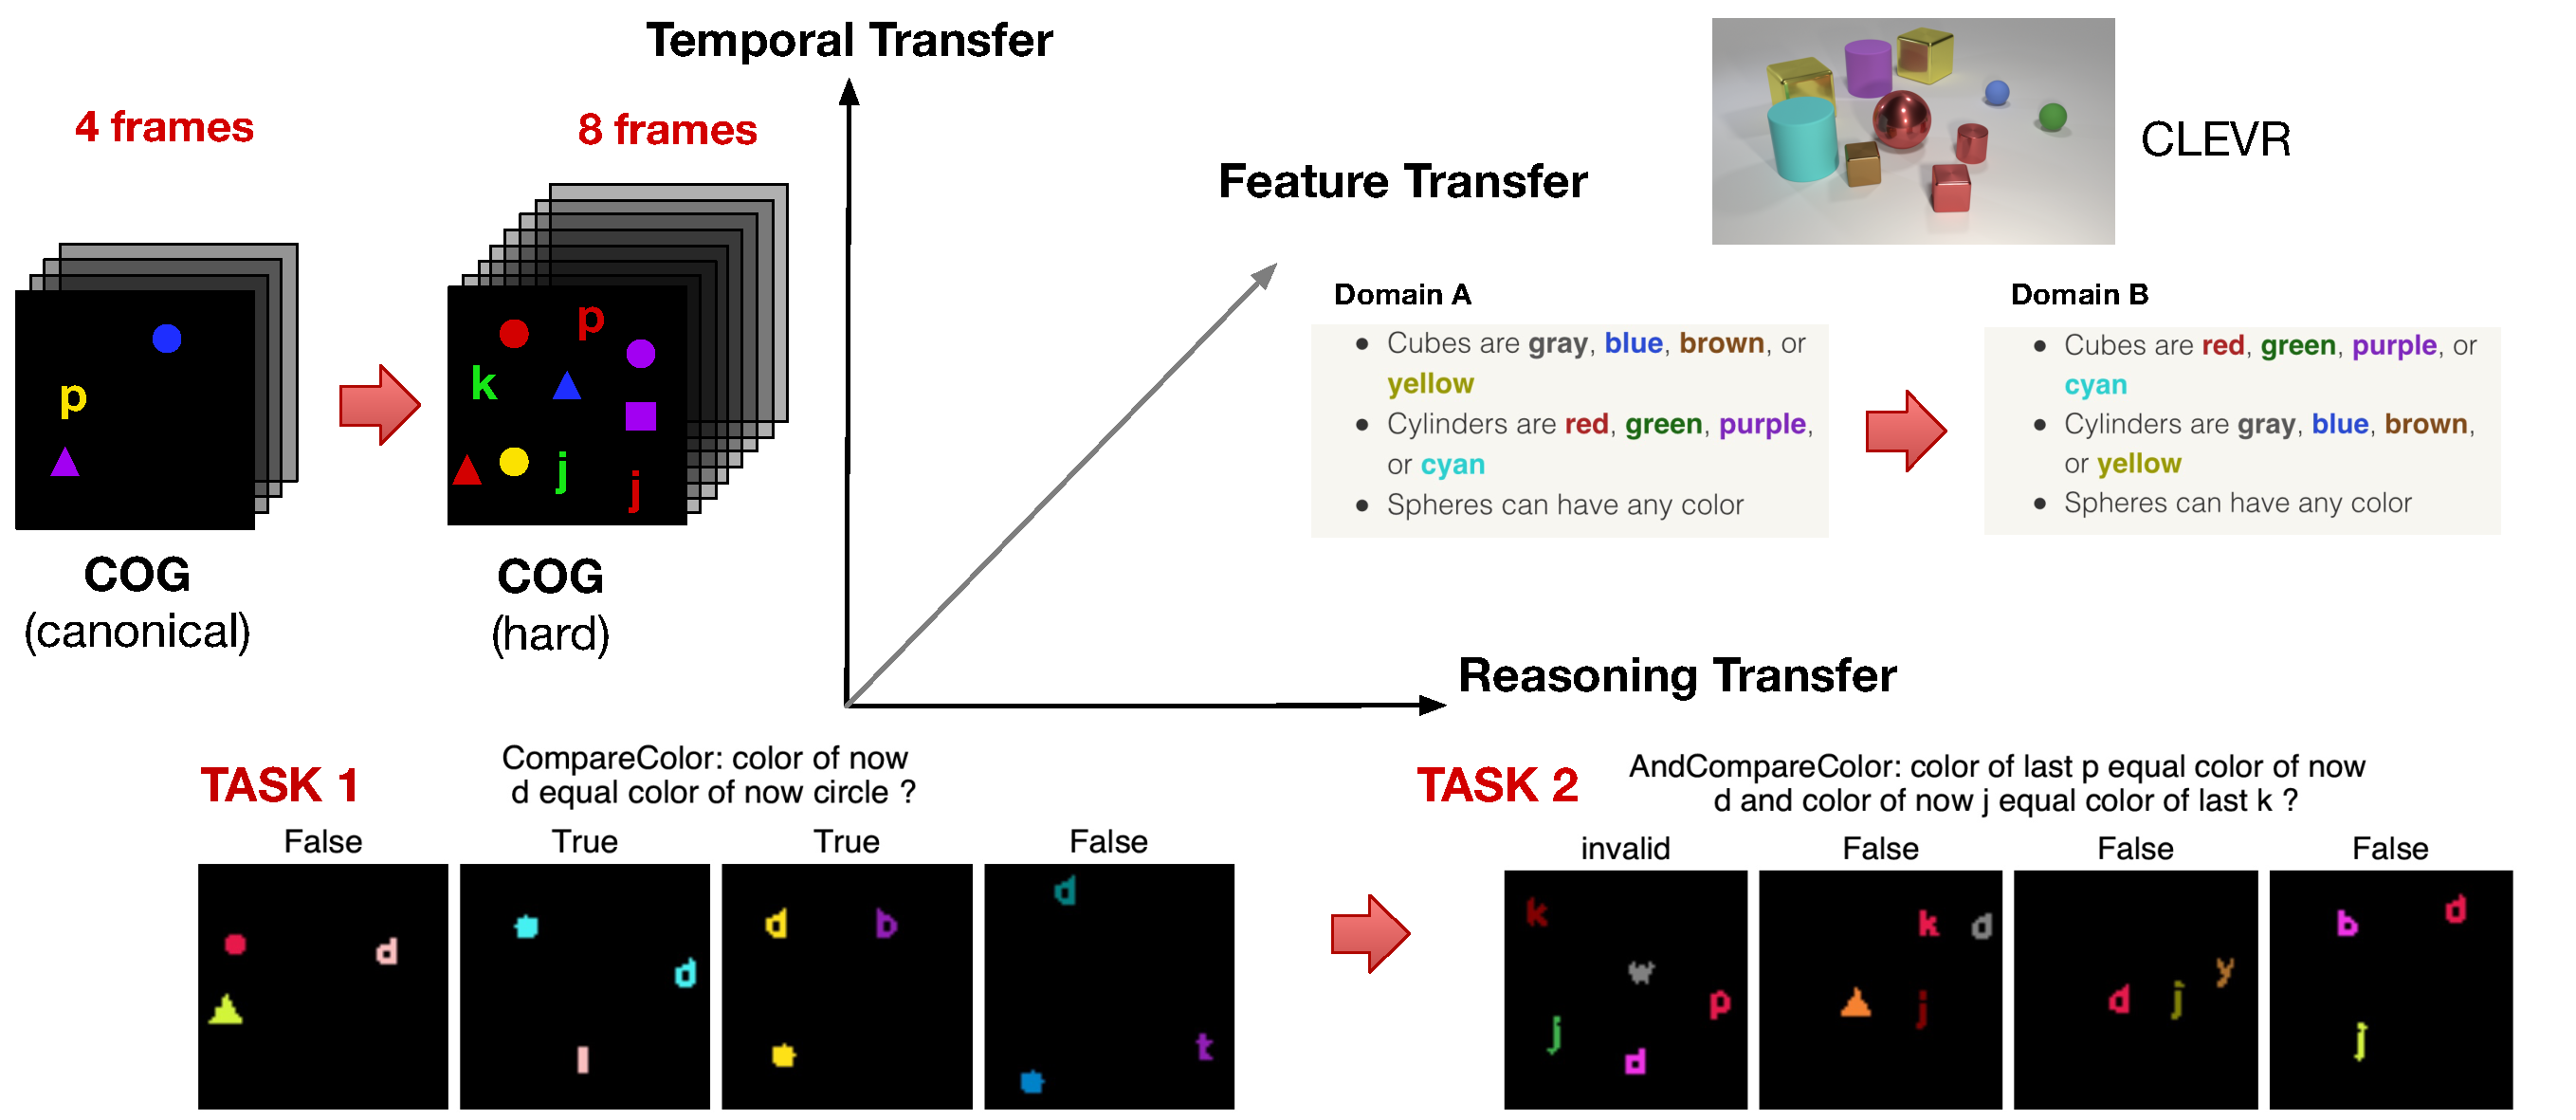
\includegraphics[width=0.9\textwidth]{../img/architecture/transfer_taxo}
	\caption{Transfer learning taxonomy.}
	\label{fig:taskonomy}\vspace{-10pt}
\end{figure*}

We now formally define 3 kinds of transfer learning problems for visual reasoning, 
namely, \emph{feature transfer}, \emph{temporal transfer}, and \emph{reasoning transfer}.
These are illustrated in~\cref{fig:taskonomy} using representative examples from CLEVR using dataset variants CoGenT-A and CoGenT-B, and COG using two dataset types: canonical and hard. These datasets were chosen because they
are particularly suited for experimental investigations of transfer learning described in the following section.
%In \cref{sec:experiments}, we detail the performance of SAMNet for each of these 3 kinds, using the CLEVR-CoGenT dataset for feature transfer, the COG dataset for temporal transfer, and finally both datasets for reasoning transfer, with appropriate baseline comparisons.
Let $\cQ$ and $\cV$ denote the set of questions and visual inputs, respectively.
The feature space is $\cQ \times \cV$ and the task is to answer
the question $q \in \cQ$ on visual input $v \in \cV$.
The output set $\cY$ is the union of legitimate answers
over all questions in $\cQ$.
\begin{description}
	%\compresslist % used to reduce spacing
	\item[Feature Transfer:] In this setting of domain adaptation, 
	the distributions $P_S$ and $P_T$ of the source and target, respectively, differ in the feature attributes such as shape, color, and size, or their combinations
	thereof.
	For example, CoGenT-A and CoGenT-B variants of CLEVR use complementary colors
	for cubes and cylinders (\cref{fig:taskonomy}), so $P_S$ and $P_T$ have disjoint support when conditioned on these shapes. This is empirically investigated in~\cref{sec:feature}.
		
	\item[Temporal Transfer:] Here we introduce a complexity measure $C(q,v)$ that reflects the ease or difficulty of answering question $q$ on 
	visual input $v$ that takes the temporal aspect of reasoning into account.
	For any $(q_S,v_S)$ and $(q_T,v_T)$ in the support of $P_S$ and $P_T$ respectively, we require that $C(q_S,v_S)$ is strictly less than $C(q_T,v_T)$.
	For example, going from the COG canonical dataset to the hard dataset, we see that there are more distracting objects in each frame and more frames to process that could cumulatively affect the ability to transfer the learned model for the canonical dataset to the hard version. This is empirically investigated in~\cref{sec:temporal}.	
	
	\item[Reasoning Transfer:]
	Here, we investigate whether the reasoning processes can be transferred in the setting where questions in the source and target domain belong to different categories.
	Fix a subset $\cQ' \subseteq \cQ$ of questions sharing a common structure.
	\Cref{fig:taskonomy} shows representative questions for two subsets with  self-explanatory names: \textit{CompareColor} and \textit{AndCompareColor}.
	Given a fixed global distribution on $\cQ \times \cV$, observe that
	$\cQ'$ induces a conditional distribution on $\cQ \times \cV$.
	Let $\cQ_S$ and $\cQ_T$ be the source and target questions, respectively; typically, $\cQ_S$ and $\cQ_T$ will be disjoint, therefore, this also holds for the support of $P_S$ and $P_T$ on the induced distribution.
	Transfer learning in this setting is most effective when the source and target questions
	share common attributes in the reasoning process. This is evidently true for \textit{CompareColor} and the more complex \textit{AndCompareColor}; the latter category involves reasoning elements that can be found in the former category. The effectiveness of reasoning transfer with respect to various combinations of source-target pairs is thoroughly investigated in~\cref{sec:reasoning-transfer-clevr} using the CoGenT-A variant of CLEVR and in~\cref{sec:reasoning-transfer-cog} using the COG canonical dataset.
	

%	\item[Temporal Transfer:] This is again a domain adaptation setting similar to feature transfer in that $\cX_S = \cX_T \subseteq \cQ \times \cV$
%	and there is a single task.
%	The key difference is that we introduce a notion of complexity $C(v) = (n, m)$ for a visual input $v$,
%	where $n$ equals the maximum number of objects $n$ in an image, and $m$
%	equals  the number of frames in a video.
%	For any visual input $v_S$ coming from $\cX_S$ with $C(v_S) = (n_S, m_S)$
%	and for any visual input $v_T$ coming from $\cX_T$ with $C(v_T) = (n_T, m_T)$, we require that $n_T \ge n_S$ and
%	$m_T \ge m_S$ with at least one inequality being a strict one.
%	Thus, we necessarily increase the complexity of the visual input going from the source to the target domain.
%	For example, going from the COG canonical dataset to the hard dataset, we see that there are more distracting objects in each frame and more frames to process that could cumulatively affect the ability to transfer the learned model for the canonical dataset to the hard version. This is empirically investigated in~\cref{sec:temporal}.
%	\item[Reasoning Transfer:]
%	This setting requires an extension of~\cref{defn:transfer} above to investigate transfer learning when
%	grouping questions into families. Let $\cV$ be the feature space consisting of visual inputs only, shared by
%	all tasks, with a common distribution $P(X)$. For each question $q \in \cQ$, we define the task
%	$\cT_q = (\cY_q, f_q(\cdot))$ where
%	the output set $\cY_q$ is the set of legitimate answers to $q$ and $f_q(v)$, for a visual input $v$,
%	is the answer to question $q$ on visual input $v$.
%	Thus, tasks are in a 1-1 correspondence with questions.
%	\Cref{fig:taskonomy} shows representative questions for two task families: \textit{CompareColor} and \textit{AndCompareColor}.
%	A \emph{task family} is a probability distribution on tasks is obtained in our case by defining the distribution on $\cQ$. T
%	
%	Given a task family, the goal is to learn a prediction function that gives an answer to $f_q(v)$ for $v \in \cV$ chosen according
%	to the feature space distribution and $q$ chosen according to the task probability distribution.
%	Suppose $\cF_S$ is the source task family and $\cF_T$ is the target task family.
%	Transfer learning aims to help improve the learning of the predictive function for the target task family
%	using the knowledge in the source task family.
%	Referring to the same example above,  
%	This is empirically investigated in~\cref{sec:reasoning-transfer-clevr} using the CoGenT-A variant of CLEVR and in~\cref{sec:reasoning-transfer-cog} using the COG canonical dataset.
\end{description}

If labeled data is available for $\cX_T$, a training algorithm distinction we make is between \emph{zero-shot learning} and \emph{finetuning}. Finetuning entails the use of labeled data in the target domain $\cD_T$, foreseeing performance gain on the target task $\cX_T$, after initial training on $\cX_S$ and additional training on $\cX_T$. Zero-shot learning thus refers to immediate test on $\cX_T$ after initial training on $\cX_S$.
